\documentclass[]{article}

\usepackage{float}
\usepackage{graphicx}
\usepackage[export]{adjustbox}

%opening
\title{Parallel System Architectures --- Lab 2}
\author{Andrea Di Dio --- 12967424}

\begin{document}

\maketitle

\section{Design Choices}

For this assignment we had to implement a split-transaction bus. My implementation is inspired by the \textit{simple\_bus} example from the SystemC documentation. There are two main components which have been added on top of the code for assignment 1 in order to implement the valid-invalid cache coherency protocol. The Bus is non-blocking and works with an arbiter to decide which request to satisfy on the falling edge on the clock. I decided to use a two-phase synchronization approach where the caches (bus masters) make the requests to the bus on the rising edge of the clock and then one request from the queue is satisfied on the falling edge of the clock. \\
The caches are connected to the bus by means of a port to allow for a TLM implementation of the components such that the caches can use two method calls (\textit{port\_bus$\rightarrow$write() or port\_bus$\rightarrow$read()}). These calls place a new \textit{bus\_sig\_t} request in the queue which represents the type of bus operation, the address and the id of the requester cache. Each cache has a separate \textit{snoop} thread, which waits for the signal driven by the bus which uses it to ``reply" to requests to change, and take different actions such as invalidating a cache line whenever a network read is observed or updating the line requested from memory.\\
The arbiter is the component that at every falling edge of the clock picks a request to be processed. Unless the queue contains a request which is ``in process" already and should therefore be prioritized to finish, the arbiter simply picks the oldest request which allows to serve the requests in FIFO order.\\
The \textit{execute} thread of the bus, tries to prioritize the replies from memory by writing to the signal as soon as the memory component (bus slave) returns the \textit{MEM\_DONE} return value. This allows the requester of that memory operation and other snooping caches to observe a change in value as soon as possible.


\section{Results --- Raw Data}

\subsection{Debug Tracefile}

\subsubsection{2 Processors}

\begin{table}[H]
	\begin{tabular}{|l|l|l|l|l|l|l|l|}
		\hline
		\textbf{CPU} & \textbf{Reads} & \textbf{RHit} & \textbf{RMiss} & \textbf{Writes} & \textbf{WHit} & \textbf{WMiss} & \textbf{Hitrate} \\ \hline
		0            & 30             & 0             & 30             & 25              & 1             & 24             & 1.818182         \\ \hline
		1            & 32             & 0             & 32             & 35              & 1             & 34             & 1.492537         \\ \hline
	\end{tabular}
\end{table}

Total Memory Accesses = 124\\
Average Bus Acquisition Time = 2331152 ps\\
Total Simulation Time = 12625 ns\\

\subsubsection{4 Processors}

\begin{table}[H]
	\begin{tabular}{|l|l|l|l|l|l|l|l|}
		\hline
		\textbf{CPU} & \textbf{Reads} & \textbf{RHit} & \textbf{RMiss} & \textbf{Writes} & \textbf{WHit} & \textbf{WMiss} & \textbf{Hitrate} \\ \hline
		0            & 8              & 0             & 8              & 8               & 1             & 7              & 6.250000         \\ \hline
		1            & 27             & 0             & 27             & 32              & 0             & 32             & 0                \\ \hline
		2            & 43             & 1             & 42             & 38              & 2             & 36             & 3.703704         \\ \hline
		3            & 45             & 0             & 45             & 42              & 0             & 42             & 0                \\ \hline
	\end{tabular}
\end{table}

Total Memory Accesses = 137\\
Average Bus Acquisition Time = 4747518 ps\\
Total Simulation Time = 13938 ns\\

\subsubsection{8 Processors}

\begin{table}[H]
	\begin{tabular}{|l|l|l|l|l|l|l|l|}
		\hline
		\textbf{CPU} & \textbf{Reads} & \textbf{RHit} & \textbf{RMiss} & \textbf{Writes} & \textbf{WHit} & \textbf{WMiss} & \textbf{Hitrate} \\ \hline
		0            & 6              & 0             & 6              & 4               & 0             & 4              & 0                \\ \hline
		1            & 34             & 0             & 34             & 22              & 0             & 22             & 0                \\ \hline
		2            & 35             & 0             & 35             & 43              & 0             & 43             & 0                \\ \hline
		3            & 39             & 2             & 37             & 46              & 2             & 44             & 4.705882         \\ \hline
		4            & 36             & 0             & 36             & 55              & 0             & 55             & 0                \\ \hline
		5            & 52             & 0             & 52             & 47              & 0             & 47             & 0                \\ \hline
		6            & 48             & 3             & 45             & 51              & 2             & 49             & 5.050505         \\ \hline
		7            & 42             & 1             & 41             & 55              & 5             & 50             & 6.185567         \\ \hline
	\end{tabular}
\end{table}

Total Memory Accesses = 153\\
Average Bus Acquisition Time = 6667932 ps\\
Total Simulation Time = 15554 ns\\

\subsection{Random Tracefile}

\subsubsection{2 Processors}

\begin{table}[H]
	\begin{tabular}{|l|l|l|l|l|l|l|l|}
		\hline
		\textbf{CPU} & \textbf{Reads} & \textbf{RHit} & \textbf{RMiss} & \textbf{Writes} & \textbf{WHit} & \textbf{WMiss} & \textbf{Hitrate} \\ \hline
		0            & 16496          & 385           & 16111          & 16402           & 393           & 16009          & 2.364885         \\ \hline
		1            & 24556          & 865           & 23691          & 24804           & 877           & 23927          & 3.529173         \\ \hline
	\end{tabular}
\end{table}

Total Memory Accesses = 85616\\
Average Bus Acquisition Time = 1610251461 ps\\
Total Simulation Time = 8647318 ns\\

\subsubsection{4 Processors}

\begin{table}[H]
	\begin{tabular}{|l|l|l|l|l|l|l|l|}
		\hline
		\textbf{CPU} & \textbf{Reads} & \textbf{RHit} & \textbf{RMiss} & \textbf{Writes} & \textbf{WHit} & \textbf{WMiss} & \textbf{Hitrate} \\ \hline
		0            & 8039           & 85            & 7954           & 8251            & 89            & 8162           & 1.068140         \\ \hline
		1            & 20450          & 0             & 20450          & 20221           & 0             & 20221          & 0                \\ \hline
		2            & 26553          & 982           & 25571          & 26498           & 1056          & 25442          & 3.841586         \\ \hline
		3            & 29600          & 0             & 29600          & 29695           & 3             & 29692          & 0.005059         \\ \hline
	\end{tabular}
\end{table}

Total Memory Accesses = 94628\\
Average Bus Acquisition Time = 3321838086 ps\\
Total Simulation Time = 9557530 ns\\

\subsubsection{8 Processors}

\begin{table}[H]
	\begin{tabular}{|l|l|l|l|l|l|l|l|}
		\hline
		\textbf{CPU} & \textbf{Reads} & \textbf{RHit} & \textbf{RMiss} & \textbf{Writes} & \textbf{WHit} & \textbf{WMiss} & \textbf{Hitrate} \\ \hline
		0            & 4113           & 22            & 4091           & 4030            & 35            & 3995           & 0.699988         \\ \hline
		1            & 18318          & 0             & 18318          & 18440           & 0             & 18440          & 0                \\ \hline
		2            & 25834          & 21            & 25813          & 25470           & 30            & 25440          & 0.099407         \\ \hline
		3            & 29549          & 1257          & 28274          & 28801           & 1180          & 27621          & 4.207369         \\ \hline
		4            & 31366          & 2             & 31364          & 30548           & 1             & 30547          & 0.004845         \\ \hline
		5            & 32015          & 12            & 32003          & 31782           & 26            & 31756          & 0.059564         \\ \hline
		6            & 32327          & 1626          & 30701          & 32285           & 1653          & 30632          & 5.074909         \\ \hline
		7            & 32536          & 1687          & 30849          & 32584           & 1771          & 30813          & 5.310197         \\ \hline
	\end{tabular}
\end{table}

Total Memory Accesses = 97930\\
Average Bus Acquisition Time = 4244396129 ps\\
Total Simulation Time = 9891031 ns\\

\subsection{FFT Tracefile}

\subsubsection{2 Processors}

\begin{table}[H]
	\begin{tabular}{|l|l|l|l|l|l|l|l|}
		\hline
		\textbf{CPU} & \textbf{Reads} & \textbf{RHit} & \textbf{RMiss} & \textbf{Writes} & \textbf{WHit} & \textbf{WMiss} & \textbf{Hitrate} \\ \hline
		0            & 29313          & 3423          & 25890          & 15417           & 2013          & 13404          & 12.152918        \\ \hline
		1            & 29262          & 3176          & 26086          & 14801           & 1897          & 12904          & 11.513061        \\ \hline
	\end{tabular}
\end{table}

Total Memory Accesses = 68809\\
Average Bus Acquisition Time = 1083535306 ps\\
Total Simulation Time = 6949810 ns\\

\subsubsection{4 Processors}

\begin{table}[H]
	\begin{tabular}{|l|l|l|l|l|l|l|l|}
		\hline
		\textbf{CPU} & \textbf{Reads} & \textbf{RHit} & \textbf{RMiss} & \textbf{Writes} & \textbf{WHit} & \textbf{WMiss} & \textbf{Hitrate} \\ \hline
		0            & 11274          & 1749          & 9525           & 6553            & 945           & 5608           & 15.111909        \\ \hline
		1            & 9417           & 1462          & 7955           & 6083            & 755           & 5328           & 14.303226        \\ \hline
		2            & 9834           & 1524          & 8310           & 5523            & 610           & 4913           & 13.895943        \\ \hline
		3            & 9881           & 1507          & 8374           & 5972            & 704           & 5268           & 13.946887        \\ \hline
	\end{tabular}
\end{table}

Total Memory Accesses = 28751\\
Average Bus Acquisition Time = 932925367 ps\\
Total Simulation Time = 2903952 ns\\

\subsubsection{8 Processors}

\begin{table}[H]
	\begin{tabular}{|l|l|l|l|l|l|l|l|}
		\hline
		\textbf{CPU} & \textbf{Reads} & \textbf{RHit} & \textbf{RMiss} & \textbf{Writes} & \textbf{WHit} & \textbf{WMiss} & \textbf{Hitrate} \\ \hline
		0            & 4956           & 1103          & 3853           & 3154            & 742           & 2412           & 22.749692        \\ \hline
		1            & 3983           & 822           & 3161           & 2890            & 544           & 2346           & 19.874873        \\ \hline
		2            & 3997           & 865           & 3132           & 2703            & 502           & 2201           & 20.402985        \\ \hline
		3            & 4043           & 858           & 3185           & 2695            & 500           & 2195           & 20.154348        \\ \hline
		4            & 4055           & 851           & 3204           & 2662            & 475           & 2187           & 19.740956        \\ \hline
		5            & 4055           & 846           & 3209           & 2733            & 510           & 2223           & 19.976429        \\ \hline
		6            & 4074           & 826           & 3248           & 2710            & 483           & 2227           & 19.295401        \\ \hline
		7            & 4124           & 831           & 3293           & 2705            & 477           & 2228           & 19.153610        \\ \hline
	\end{tabular}
\end{table}

Total Memory Accesses = 12788\\
Average Bus Acquisition Time = 533288298 ps\\
Total Simulation Time = 1291690 ns\\


\section{Experiments}

In order to show how the hitrates change by disabling snooping in the caches, I have decided to run the tests only for the 8 processor FFT tracefile as it has the more realistic access patterns.\\
My hypothesis is that disabling snooping will result in a higher hitrate, albeit being a ``fake" hitrate due to the fact that the caches will lose coherency.

\begin{figure}[H]
	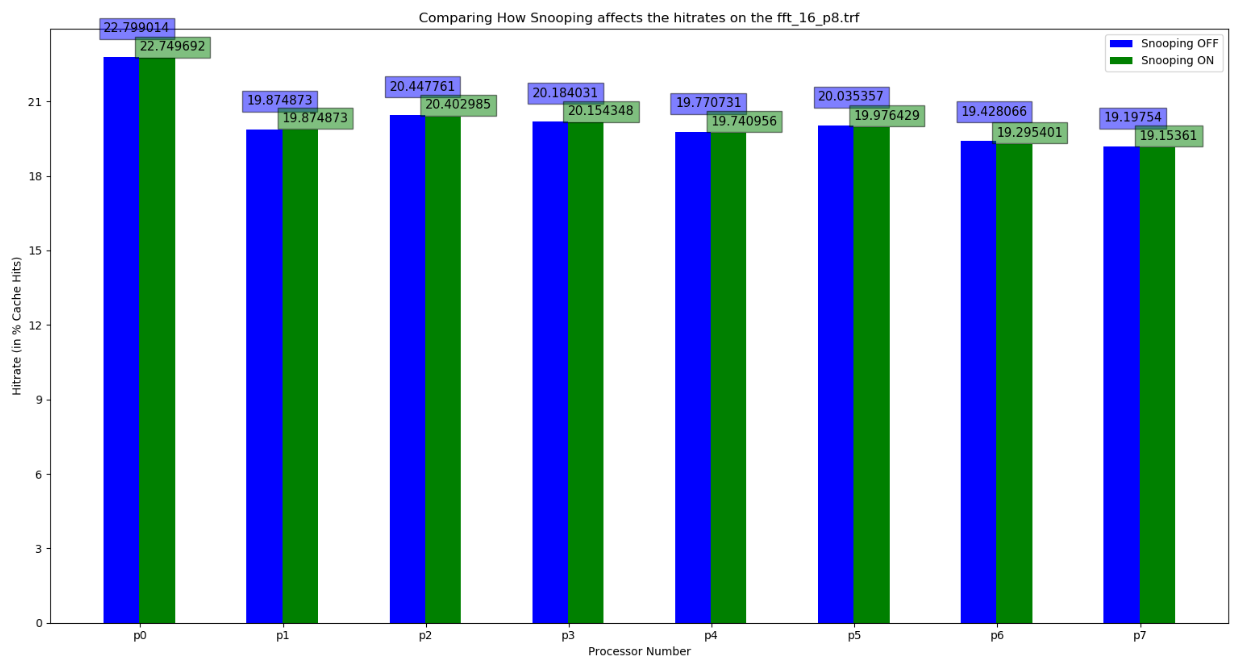
\includegraphics[scale=0.35,left]{./snoop.png}
\end{figure}


The figure above shows that disabling snooping, unexpectedly, does not increase the hitrates by much, but only marginally. One explanation for this could be that the tracefile generates access patterns which are processor independent. I.e., lines that are used by one processor are not used much in other processors, meaning that the writes don't necessarily affect the validity of the cahce lines in other CPUs.


\end{document}




